\chapter{Computation of subgraph similarity}

	In this chapter we present four different theoretical algorithms to compute subgraphs similarity as previously defined: an exhaustive enumeration, two similar randomized approach using the tools described in the previous chapter and a naive randomized approach.\medskip
	
	In the following algorithms, we will make use of parallel instructions, but we leave the specific programming choices and the comparison among the different approaches in the next chapter.
	
% \section{Calculation of indices}
%%%%%%%%%%%%%%%%%%%%%%%%%%%%%%%%%%%%%%%%%%%%%%%%%%%%%%%%%%%%%%%%%%%%%%%%%%%%%%%%%%%%%%%%%%%%%%%%%%%%%%%%%%%%%%%%%%%%
%%%%%%%%%%%%%%%%%%%%%%%%%%%%%%%%%%%%%%%%%%%%%%%%%%%%%%%%%%%%%%%%%%%%%%%%%%%%%%%%%%%%%%%%%%%%%%%%%%%%%%%%%%%%%%%%%%%%
\section{Indices calculation}

Now we illustrate the procedures to calculate the Frequency Jaccard and Bray-Curtis indices, as they are independent from the next algorithms we will present.\medskip

As previously seen, instead of iterate over all the strings in $\Sigma^{q}$ we can restrict to $\mathcal{L} \subseteq \Sigma^{q}$, the set of all possible $q$-grams found in the $q$-paths of $G$. 

An additional improvement can be made: if we want to calculate the similarity between two set $A, B \subset V$ it is enough to ranging, instead over $\mathcal{L}$, over $\mathcal{W} = \{ x \in \Sigma^{q} : x \in L(A) \text{ or } x \in L(B) \} \subseteq \Sigma^{q}$, as we can easily see that for any $x \in ( \Sigma^{q} \setminus \mathcal{W} )$ both $f_A[x]$ and $f_B[x]$ are equal to zero.\medskip

A last note, we can observe that in the Frequency Jaccard index we don't have to explicitly calculate $f_{A \cup B}[x]$ and its summary, as the exact value of $R = \Sigma_{x \in \mathcal{W}} f_{A \cup B}[x]$ can be easily calculate from $f_{A}[x] \text{ and } f_{B}[x]$.\medskip

So we define the following procedures based on \eqref{bray-sub} and \eqref{jaccard-sub}:\medskip

\begin{algorithm}[h]
	\small
	\DontPrintSemicolon
	\SetKwInOut{Input}{Input}
	\SetKwInOut{Output}{Output}
	\Input{$\mathcal{W} = $ dictionary of $q$-grams\\$f_{A}[x] = $ frequency of each $x \in \mathcal{W}$ in $A$\\$f_{B}[x] = $ frequency of each $x \in \mathcal{W}$ in $B$}
	\Output{$BC(A,B) = $ the similarity between $A$ and $B$ according to Bray-Curtis index}
	\BlankLine
	$num \gets 0$\;
	$den \gets 0$\;
	\ForEach{$x \in \mathcal{W}$}{
		$num \gets num + 2 \times \min( f_{A}[x], f_{B}[x] )$\;
		$dem \gets den + f_{A}[x] + f_{B}[x]$\;
	}
	$BC \gets \frac{num}{den}$\;
	\Return{$BC$}
	\caption{\textsc{Bray-Curtis}}
	\label{alg:bray-curtis}
\end{algorithm}

\begin{algorithm}[h]
	\small
	\DontPrintSemicolon
	\SetKwInOut{Input}{Input}
	\SetKwInOut{Output}{Output}
	\Input{$\mathcal{W} = $ dictionary of $q$-grams\\$f_{A}[x] = $ frequency of each $x \in \mathcal{W}$ in $A$\\ $f_{B}[x] = $ frequency of each $x \in \mathcal{W}$ in $B$\\ $R =$ summation of all frequency}
	\Output{$FJ(A,B) = $ the similarity between $A$ and $B$ according to Frequency Jaccard index}
	\BlankLine
	$num \gets 0$\;
	\ForEach{$x \in \mathcal{W}$}{
		$num \gets num + \min( f_{A}[x], f_{B}[x] )$\;
	}
	$FJ \gets \frac{num}{R}$\;
	\Return{$FJ$}
	\caption{\textsc{Frequency-Jaccard}}
	\label{alg:jaccard}
\end{algorithm}

Algorithm 1 and 2 calculate the values of $BC(A,B)$ and $FJ(A,B)$, as previously defined, by ranging over the given dictionary of $q$-grams $\mathcal{W}$.

\begin{lemma}
	The execution of \textsc{Bray-Curtis} or \textsc{Frequency-Jaccard} requires $O(|W|)$ time and $O(1)$ space. 	
\end{lemma}

In the next algorithms we will focus to compute the values of $\mathcal{W}$, $f_{A}$, $f_{B}$ and $R$.

\clearpage 
%%%%%%%%%%%%%%%%%%%%%%%%%%%%%%%%%%%%%%%%%%%%%%%%%%%%%%%%%%%%%%%%%%%%%%%%%%%%%%%%%%%%%%%%%%%%%%%%%%%%%%%%%%%%%%%%%%%%
%%%%%%%%%%%%%%%%%%%%%%%%%%%%%%%%%%%%%%%%%%%%%%%%%%%%%%%%%%%%%%%%%%%%%%%%%%%%%%%%%%%%%%%%%%%%%%%%%%%%%%%%%%%%%%%%%%%%
\section{Naive approach}

	The naive approach consists in enumerate all the possible $q$-grams of simple $q$-paths leading to $u \in A \cup B$. 
	This can be done by starting an exhaustive search for each $u \in A \cup B$.
	
    \begin{algorithm}[h]
    \small
    \DontPrintSemicolon
    \SetKwInOut{Input}{Input}
    \SetKwInOut{Output}{Output}
    \Input{$q = $ length of the paths\\$A, B = $ set of nodes to compare}
	\Output{$\mathcal{W} = $ dictionary of $q$-grams\\$f_{A}[x] = $ frequency of each $x \in \mathcal{W}$ in $A$\\ $f_{B}[x] = $ frequency of each $x \in \mathcal{W}$ in $B$\\ $R =$ summation of all frequency}
    \BlankLine
    $R \gets 0$\;
	$\mathcal{W} \gets \emptyset$\;
	$f_{A \cup B} \gets \emptyset$ \quad \;    
	$f_{A} \gets \emptyset$\; 
	$f_{B} \gets \emptyset$\; 
	\BlankLine
    \textbf{parallel} \ForEach{$u \in A \cup B$}{
		$\langle \mathcal{W}_{u}, f_{u} \rangle \gets \textsc{ExhaustiveSearch}(\langle u \rangle, q)$\;
		$\mathcal{W} \gets \mathcal{W} \cup \mathcal{W}_{u}$\;
		$f_{A \cup B} \gets f_{A \cup B} \cup f_{u}$\;
	}
	\BlankLine    
	\ForEach{$\langle u, x \rangle \in f_{A \cup B}$}{ 
		$R \gets R + f_{A \cup B}[\langle u, x \rangle]$\;
		\If{$u \in A$}{
			$f_{A}[x] \gets f_{A}[x] + f_{A \cup B}[\langle u, x \rangle]$\;
		}
		\If{$u \in B$}{
			$f_{B}[x] \gets f_{B}[x] + f_{A \cup B}[\langle u, x \rangle]$\;
		}
	}
	\BlankLine
    \Return{$\langle \mathcal{W}$, $f_{A}$, $f_{B}$, $R \rangle$}
    \caption{\textsc{brute-force}}
    \label{alg:brute-force}
    \end{algorithm}

	Here we define $\mathcal{W}_{u}$ and $f_{u}$ as, respectively, the dictionary and the frequency of $q$-grams of the $q$-paths leading to the node $u \in A \cup B$.
	 
	Thus we calculate $\mathcal{W}$ with the property $\mathcal{W} = \Sigma_{u \in A \cup B}{\ \mathcal{W}_{u} }$ and, in the same way, $f_{A \cup B}$ with the property
	$f_{A \cup B} = \Sigma_{u \in A \cup B}{\ f_{u} }$.
	
	The value of R is calculated as we defined it in the beginning of the chapter $R = \Sigma_{x \in \mathcal{W} }{\ f_{A \cup B}[x] }$.

	At last, we can calculate the value of $f_{A}$ and $f_{B}$ from $f_{A \cup B}$ by looking at the leading nodes and separate the frequencies, 
	depending if it belong to $A$, $B$ or both.

	Note that, as we have to separate the frequencies between $f_{A}$ and $f_{B}$, the type of $f_{A \cup B}$ is not a map $ \Sigma^{q} \rightarrow \mathbb{N}$
	but instead is a map $V \times \Sigma^{q} \rightarrow \mathbb{N}$, where the element in $V$ is the leading node of the $q$-path associated to the $q$-gram.\medskip
	
	The values of $FJ(A,B)$ and $BC(A,B)$ calculated using this method are exact, we will use it only to compare the precision of the following approaches as it found all the possible $O(|\Sigma|^{q})$ $q$-gram with a complexity of $O(|V|^{q})$.\medskip
	
	For completeness we also illustrate the $\textsc{ExhaustiveSearch}$ algorithm that keeps track of the current $q$-path and its relative $q$-gram.
	
    \begin{algorithm}[h]
		\small
		\DontPrintSemicolon
		\SetKwInOut{Input}{Input}
		\SetKwInOut{Output}{Output}
		\Input{$\pi = \langle u_{1}, \ldots, u_{|\pi|} \rangle $ current traversing path of length $\leq q$ \\$q = $ length of the paths }
		\Output{$\mathcal{W} =$ dictionary of $q$-grams of $q$-path having $\pi$ as suffix\\$f_{u}[\langle u_{q}, x \rangle] = $ frequency of each $x \in \mathcal{W}$ leading to $u_{q}$}
		\BlankLine
		$\mathcal{W} \gets \emptyset$\;
		$f_{u} \gets \emptyset$ \quad \;    
		\BlankLine
		\If{$|\pi| = q$}{
			$\mathcal{W} \gets \{ L(\pi) \}$\;
			$f_{u}[\langle u_{q}, L(\pi) \rangle] \gets 1$\;
		}
		\Else{
			\ForEach{$v \in N(u_{1}) \setminus \pi$}{
				$\langle \mathcal{W}_{v}, f_{v} \rangle \gets \textsc{ExhaustiveSearch}(\langle v \rangle \cdot \pi, q)$\;
				$\mathcal{W} \gets \mathcal{W} \cup \mathcal{W}_{v}$\;
				$f_{u} \gets f_{u} \cup f_{v}$\;
			}	
		}
		\BlankLine
		\Return{$\langle \mathcal{W}$, $f_{u} \rangle$}
		\caption{\textsc{ExhaustiveSearch}}
		\label{alg:exhaustive-search}
	\end{algorithm}

	Where the symbol $\cdot$ is the concatenation of paths, note that we put the node $v$ before the path $\pi$ as we are interested to find all the $q$-path leading to the original calling node $u$.\medskip
	
	In Algorithm 4, when path $\pi$ is a complete $q$-path, we have the base case of the recursion that simply returns $\mathcal{W} = \{ L(\pi) \}$, 
	the dictionary composed only by the label of $\pi$, and the frequency $f_{u}[\langle u_{q}, L(\pi) \rangle] = 1$ as we have only one path.
	
	When the path $\pi$ is not completed we recursively visit all its neighbor, with the new path obtained by prepending the node $v$ to the current path $\pi$.\medskip
	
	\clearpage
	
	As last thing, with $N(u_{1}) \setminus \pi$ we avoid to revisit the nodes already in the path $\pi$, in this way we restrict the searching only on the simple $q$-paths.
	
	\begin{lemma}
		For any two sets of nodes $A, B \subseteq V$, the running time of \textsc{brute-force} requires $O(|V|^{q})$ time and $O(\mathcal{L}) = O(|\Sigma|^{q})$ space.
	\end{lemma}

	Now we present a little example to better understand:
	
	\begin{esempio}
		We want to compute the similarity between the two nodes $4$ and $3$ in the following graph.	
	\end{esempio}


%	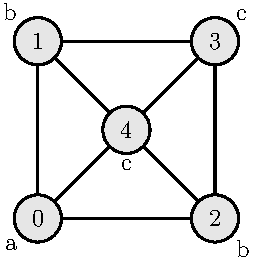
\includegraphics[width=0.30\textwidth]{figure/figure-3-2}

%	\begin{minipage}{0.95\textwidth}\raggedright
	
%		\begin{wrapfigure}{R}{0.3\textwidth}
		% \centering
%		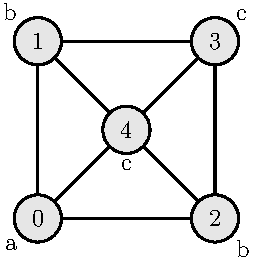
\includegraphics[width=0.40\textwidth]{figure/figure-3-2}
%		\end{wrapfigure}

		
		\begin{wrapfigure}{R}{0\textwidth}
		%	\centering
			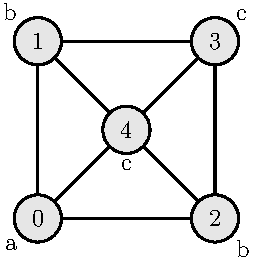
\includegraphics[width=0.35\textwidth]{figure/figure-3-2}
		\end{wrapfigure}
	
		$\textsc{ExhaustiveSearch}(4, 3)$ return: \medskip

		$\mathcal{W}_{4} = \{ abc, bac, bbc, cbc \}$ \medskip
		
		$f_{4}[\langle 4, abc \rangle] = 2$ ($\textsc{3-1-0}$ $\textsc{4-1-0}$ $\textsc{3-2-0}$ $\textsc{4-2-0}$)\medskip
		
		$f_{4}[\langle 4, bac \rangle] = 2$ ($\textsc{1-4-0}$ $\textsc{2-4-0}$)\medskip
		
		$f_{4}[\langle 4, bbc \rangle] = 2$ ($\textsc{3-4-0}$)\medskip
		
		$f_{4}[\langle 4, cbc \rangle] = 2$ ($\textsc{3-4-0}$)\bigskip
		
		$\textsc{ExhaustiveSearch}(3, 3)$ return:\medskip
		
		$\mathcal{W}_{3} = \{ abc, acc, bcc, cbc \}$\medskip
		
		$f_{3}[\langle 3, abc \rangle] = 2$ ($\textsc{0-1-3}$, $\textsc{0-2-3}$)\medskip
		
		$f_{3}[\langle 3, acc \rangle] = 1$ ($\textsc{0-4-3}$)\medskip
		
		$f_{3}[\langle 3, bcc \rangle] = 2$ ($\textsc{1-4-3}$, $\textsc{2-4-3}$)\medskip
		
		$f_{3}[\langle 3, cbc \rangle] = 2$ ($\textsc{4-1-3}$, $\textsc{4-2-3}$)\bigskip
		
		So the dictionary $\mathcal{W}$ is: \medskip
		
		$\mathcal{W} = \mathcal{W}_3 \cup \mathcal{W}_4 = \{ abc, acc, bac, bbc, bcc, cbc \}$\bigskip
		
		The similarity according to the two indices is: \medskip

		$BC(\{3\}, \{4\}) = \frac{2 \times ( 2 + 0 + 0 + 0 + 0 + 2 ) }{ 4 + 1 + 2 + 2 + 2 + 4 } = \frac{8}{15}$ \medskip
		
		$FJ(\{3\}, \{4\}) = \frac{ 2 + 0 + 0 + 0 + 0 + 2 }{ 4 + 1 + 2 + 2 + 2 + 4 } = \frac{4}{15}$ \medskip
		
%	\end{minipage}
%	\begin{minipage}{0.30\textwidth}
%		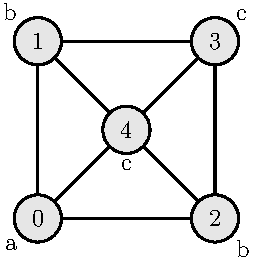
\includegraphics[width=\linewidth]{figure/figure-3-2}
%	\end{minipage}
			
\clearpage

%%%%%%%%%%%%%%%%%%%%%%%%%%%%%%%%%%%%%%%%%%%%%%%%%%%%%%%%%%%%%%%%%%%%%%%%%%%%%%%%%%%%%%%%%%%%%%%%%%%%%%%%%%%%%%%%%%%%
%%%%%%%%%%%%%%%%%%%%%%%%%%%%%%%%%%%%%%%%%%%%%%%%%%%%%%%%%%%%%%%%%%%%%%%%%%%%%%%%%%%%%%%%%%%%%%%%%%%%%%%%%%%%%%%%%%%%
\section{Efficient computation}

The main hurdle of the problem is to compute the frequency map $f_{X}[\ ]$ for some sets $X \in V$,
as it can grow up to have a size of $|\Sigma|^{q}$ and its definition requires to explore $|V|^{q}$ $q$-paths.\medskip

We present a random estimator based on color coding and sketching with the property that it can be computed
efficiently even on big networks and its expected value is the actual similarity index~\cite{SubSim}.\medskip

As first thing using the color coding we reduce the number of potentially explored $q$-paths from $|V|^{q}$ to $2^{O(q)}|V|$, 
thus making it feasible for large value of $|V|$ and with $q = O(\log |V|)$.

Second, instead of calculate the correct value of $f_{X}[\ ]$ we computing its sketch with a size small compared to $|\Sigma|^{q}$,
which is a significant benefit when $|\Sigma|$ or $q$ are large.

%%%%%%%%%%%%%%%%%%%%%%%%%%%%%%%%%%%%%%%%%%%%%%%%%%%%%%%%%%%%%%%%%%%%%%%%%%%%%%%%%%%%%%%%%%%%%%%%%%%%%%%%%%%%%%%%%%%%
%%%%%%%%%%%%%%%%%%%%%%%%%%%%%%%%%%%%%%%%%%%%%%%%%%%%%%%%%%%%%%%%%%%%%%%%%%%%%%%%%%%%%%%%%%%%%%%%%%%%%%%%%%%%%%%%%%%%
\subsection*{$preprocess(G,q)$: Color coding of the $q$-paths}

Now we illustrate how to preprocessing the input graph $G=(V,E)$ given an integer $q > 0$, in particular we restrict our attention to $q = O(\log |V|)$.

Note that the preprocessing is independent from the labeling function $L$ and from the subsets $A,B$ to compare, 
as it depends only from the graph $G$ and the value of $q$, so we can execute the preprocessing once and 
then reuse the color coding table for different values of $A,B$ or even $L$.\medskip

\begin{algorithm}[h]
	
	\small
	\DontPrintSemicolon
	\SetKwInOut{Input}{Input}
	\SetKwInOut{Output}{Output}
	\Input{$G = (V,E)$ undirected graph with $q$ random colors.}
	\Output{$M = $ dynamic programming table for color coding.}
	\BlankLine
	\textbf{parallel} \lForEach{$u \in V$}{$M_{1,u} = \langle \chi(u), 1 \rangle$}
	\BlankLine
	\For{$i \in \{ 2, 3, \ldots, q\}$}{
		\textbf{parallel} \ForEach{$u \in V$}{
			\ForEach{$v \in N(u)$}{
				\ForEach{$\langle C, f \rangle \in M_{i-1,v}$ such that $\chi(u) \not \in C$}{
					$f' \gets M_{i,u}\left(C \cup \{\chi(u)\}\right)$\;
					$M_{i,u} \gets \langle C \cup \{\chi(u)\}, f' + f \rangle$\;
				}
			}
		}   
	}
	\Return{$M$}	
	\caption{\textsc{preprocess}: \textsc{color-coding}}
	\label{alg:color-coding}
\end{algorithm}

The goal is to list all the colorful $q$-paths in $G$ using a dynamic programming approach.\medskip

First of all we assign a random coloring $\chi : V \rightarrow [q]$, so each node $u \in V$ has a color $\chi(u)$ independently and uniformly chosen from $[q]$.
Algorithm 5 build and return a table $M$ of size $q \times |V|$ 
where $M_{i,j}$ stores the collection of pairs $\langle C, f \rangle$ where  $C \subseteq [q]$ is a color set such $|C| = i$ and there are $f$ colorful $i$-paths leading to the node $j$.\medskip

Our assumption that $q = O(\log |V|)$ allows us to implement, using bit manipulations, operations on color sets in $O(1)$ time as they fits in a machine words.\medskip

Note that each entry $M_{i, j}$ contains at most $\binom{q}{i}$ sets, each with $i$ colors.
Hence the computation of the row $i$ can be done in parallel as it depends only from the row $i-1$ and require $O(|E|\ \binom{q}{i-1})$ time (as we scan all the adjacency list).
The entire computation requires thus $O(|E|\ \Sigma_{i=1}^{q}{\binom{q}{i-1}}) = O(|E|\ 2^{q})$ time.\medskip

For what concern space, the table $M$, as we already told, have a total of $q \times |V|$ entry, each of which contains at most $\binom{q}{i}$ pairs $\langle C, f \rangle$.

Each pair can be stored in $O(1)$ as they are simply $2$ integer, we have a total size of $O(\Sigma_{i=1}^{q}{\Sigma_{j=1}^{|V|}{ \binom{q}{i}}}) = O(|V|\ \Sigma_{i=1}^{q}{\binom{q}{i}}) = O(|V|\ 2^{q})$.

\begin{lemma}
	Given an undirected graph $G=(V, E)$ random colored in $[q]$, where $q = O(\log |V|)$, Algorithm 5 (preprocess($G$,$q$))
	returns the dynamic programming table $M$ of color coding in $O(|E|\ 2^{q})$ time and $O(|V|\ 2^{q})$ space. 
\end{lemma}

It is not difficult to modify the Algorithm 5 to list also the colorful $q$-grams, printing $L(\pi)$ for each colorful $q$-path $\pi$.
This makes the algorithms inefficient, indeed we still have to face with the problem that $\mathcal{L} \sim \Sigma^{q}$.\medskip

So we will pass to the next step.

%%%%%%%%%%%%%%%%%%%%%%%%%%%%%%%%%%%%%%%%%%%%%%%%%%%%%%%%%%%%%%%%%%%%%%%%%%%%%%%%%%%%%%%%%%%%%%%%%%%%%%%%%%%%%%%%%%%%
%%%%%%%%%%%%%%%%%%%%%%%%%%%%%%%%%%%%%%%%%%%%%%%%%%%%%%%%%%%%%%%%%%%%%%%%%%%%%%%%%%%%%%%%%%%%%%%%%%%%%%%%%%%%%%%%%%%%
\subsection*{$query(A,B)$: Sampling and sketching colorful paths}

Now using the color coding table $M$, and given two set of nodes $A, B$, 
we want to approximate the values of $BC(A,B)$ and $FJ(A,B)$.\medskip

As already told, we can't explore all the colorful $q$-grams, so our idea is to 
construct a sketch of $\mathcal{L}$, without explicitly calculate it, 
by sampling $r$ $q$-paths from $M$, where $r < |\mathcal{L}|$ is a user-selectable parameter.

We will use the method of the bottom-$k$ sketch by taking, without repetition, the first $r$ $q$-paths. \medskip

Our algorithm for $\textsc{query}(A,B)$ consist of three phases as follows:

\begin{itemize}
	\item Compute a suitable sketch $W \subset \mathcal{L}$ such $\tau = |W|$ is at most $r$, by sampling colorful $q$-paths using $M$.
	\item Compute $R$ and $f_{A}[x]$, $f_{B}[x]$ for each $x \in W$.
	\item Approximate $BC(A,B)$ as $BC_{W}(A,B)$ and $FJ(A,B)$ as $FJ_{W}(A,B)$.
\end{itemize}

Where $BC_{W}(A,B)$ and $FJ_{W}(A,B)$ are defined as:

\begin{equation}\label{bc-w}
	BC_{W}(A,B) = \frac{ 2 \times \Sigma_{x \in W} \min(f_{A}[x], f_{B}[x]) }{ \Sigma_{x \in W} f_{A}[x] + f_{B}[x] }
\end{equation}

\begin{equation}\label{fj-w}
	FJ_{W}(A,B) = \frac{ \Sigma_{x \in W} \min(f_{A}[x], f_{B}[x]) }{ \Sigma_{x \in W} f_{A \cup B}[x] }
\end{equation}

\subsection*{Phase 1: Colorful sampler}

Sampling uniformly using a dynamic programming approach is a topic already covered in literature, e..g Martin Dyer in ~\cite{Dyer:2003:ACD:780542.780643} or Eric Vigoda in ~\cite{Vigoda2010LectureNO},
in particular we are interested in sampling $r$ $q$-grams from colorful $q$-paths, leading to nodes belonging to $X$, using the color coding table $M$.\medskip

In particular the sample depends on the frequencies of the $q$-grams ending in $x \in X$,
as in the case of consistent weighted sampling, where more frequent $q$-grams need to be sampled more ofter.
As we don't know a priori the frequency of $q$-grams before sampling, 
we can extract the $q$-paths by looking the frequencies of colorful $q$-paths in $M$. 
We know that the number of colorful $q$-paths ending in $v$ is $M_{q,v}([q])$, 
so we extract the starting node $x \in X$ of our weighted random $q$-paths with a probability:

\begin{equation}
	p_{X}(v) = \frac{ M_{q,v}([q]) }{ \Sigma_{x \in X}{M_{q, x}([q])} }
\end{equation}

And then generating a random $q$-path by scanning the color coding table $M$ 
backward from $q-1$ to $1$, choosing nodes with a probability similar to $p_{X}(v)$
(except that during step $i$ we look at row $i$ and in the complementary of the color set of the current $i$-path).

We define out sampling algorithm as: \clearpage

\begin{algorithm}[h]
	\small
	\DontPrintSemicolon
	\SetKwInOut{Input}{Input}
	\SetKwInOut{Output}{Output}
	\Input{$X =$ multiset of nodes from graph $G$\\$M =$ color coding table for $G$\\$r =$ number of colorful paths to sample.}
	\Output{$W = $ random sample set of colorful $q$-grams of $q$-paths leading to $x \in X$ with probability $p_X(x)$.}
	\BlankLine
	$R \gets \{\}$\;
	\BlankLine
	\textbf{parallel} \For{$j\in [r]$}{
		$u\gets$ randomly chosen $v \in X$ with probability~$p_v = \frac{M_{q,v}([q])}{\sum_{z\in X} M_{q,z}([q])}$\label{line:sample}\;
		$\pi\gets \textsc{random-path-to}(u)$\;
		\lIf{$\pi\not\in R$}{$R \gets R \cup \{ \pi \}$}
		\lElse{$j\gets j-1$ \quad //repeat the step}
	}
	\BlankLine
	\Return{$W = \{ L(\pi) : \pi \in R \}$}
	\BlankLine
	\caption{\textsc{colorful-sampler}}
	\label{alg:colorful-sampler}
\end{algorithm}

And \textsc{random-path-to} is defined as:

\begin{algorithm}[h]
	\small
	\DontPrintSemicolon
	\SetKwInOut{Input}{Input}
	\SetKwInOut{Output}{Output}
	\Input{$M =$ color coding table for $G$\\$u = $ leading node of the path }
	\Output{$\pi = $ random colorful path }	
	\SetKwProg{myproc}{Function}{}{}
	$P\gets \langle u \rangle$\;
	$D\gets [q] \setminus \{\chi(u)\}$\;
	\For{$i \in \{q-1,\ldots, 1\}$}{
		%Let $N$ be the neighbors $v$ of $u$ s.t. $M[i][v]$ contains the set of colors $D$\;
		$u\gets$ randomly chosen $v \in N(u)$ with probability~$p_{v} = \frac{M_{i,v}(D) }{ \sum_{z\in N(u)} M_{i,z}(D)}$\;
		$P\gets u \cdot P$\;
		$D\gets D\setminus \{\chi(u)\}$\;
	}
	\Return{P}   
	\caption{\textsc{random-path-to}}
	\label{alg:random-path-to}
\end{algorithm}

Note that the method $\textsc{random-path-to}$ always find a colorful $q$-path,
as we at each step select only between the nodes that lead us to a colorful $q$-path
(i.e. the probability $p_{v}$ is $0$ for nodes that don't lead to a colorful $q$-path).
This property is guaranteed by the way the color coding table $M$ is generated by Algorithm 5.

\begin{lemma}
	For any multiset of nodes $X$, 
	Algorithm 6 return a random sample $W \subset |\Sigma^{q}|$ and the map frequency $f_{X}[x]$
	with a complexity of $O(rq)$ both in time and space, 
	where $q = O(\log |V|)$ and $r < |\mathcal{L}| \leq |\Sigma|^{q}$.
\end{lemma}

\clearpage
\subsection*{Phase 2: Frequency count}

Now that we have a sample $W$ composed by colorful $q$-grams, of a suitable size, 
we are interested, for a multiset of nodes $X$, in calculate $f_{X}[x]$ for each $x \in W$.
Algorithm 8, for steps $i = 1, 2, \ldots, q$, proceed by expanding in $BFS$ order only the
$i$-paths ending in a node $u \in X$ and having $i$-grams that are suffixes of $W$
(this operation can be made more space efficient by using tries or by a binary search in a set of strings).\medskip

We maintain a multiset $T$ of these $i$-grams, each represented by a triple $\langle z, x, C \rangle$
to indicate that exists a $i$-path starting from z and leading to a node $u \in X$ whose $i$-gram is $x$
and its colorset is $C$ (note that the same triple triple $\langle z, x, C \rangle$ can appear more times in $T$ 
as there might exist multiple path from $z$ to $u$ labeled with the same $i$-gram $x$).\medskip

Also in this case, considering that the computation for the $i$-grams depends only by the $(i-1)$-grams,
we can parallelize the operations for the triple with same length $i$.

\begin{algorithm}[h]

\small
\DontPrintSemicolon
\SetKwInOut{Input}{Input}
\SetKwInOut{Output}{Output}
\Input{$X =$ multiset of nodes from graph $G$\\$W = $ sample of its colorful $q$-grams}
\Output{$f_X[x] = $ frequency of each $x \in W$}
\BlankLine
$T\gets[\,]$ \quad // step~$i=1$\; 
\BlankLine
\textbf{parallel} \ForEach{$u \in X$ such that $L(u)$ appears at the end of a $q$-gram in $W$}{
	$T \gets T \cup [\langle u, L(u), \{\chi(u) \} \rangle]$\;
}
\BlankLine
\For{$i \in \{ 2, 3, \ldots, q\}$}{
	$T' \gets [\,]$\;
	\textbf{parallel} \ForEach{$\langle z, x, C \rangle \in T$}{
		\ForEach{$v \in N(z)$ such that $\chi(v) \not \in C$}{
			\If{$L(v) \cdot x$ is a suffix of a $q$-gram in $W$}{
				$T' \gets T' \cup [\langle v, L(v) \cdot x, C \cup \{\chi(v)\} \rangle]$\;
			}
		}
	}   
	$T \gets T'$\;
}
\BlankLine
$f_X \gets (0,\ldots,0)$\;
\lForEach{$\langle z, x, C \rangle \in T$}{
	$f_X[x] \gets f_X[x]+1$
}
\BlankLine
\Return{$f_X$}
\BlankLine
\caption{\textsc{f-count}: exactly counting frequencies of sampled $q$-grams}
\label{alg:f-count}
\end{algorithm}

\clearpage

It may happen that, in some big instance, Algorithm 8 
can explore many colorful paths as it expands the paths in the $X \cup N^{<q}(X)$ nodes.

To alleviate this issue we present a modified version of the Algorithm 6,
that we call $\textsc{f-samp}$, that estimate the value of $f_{X}[x]$ after having computed the sketch.\medskip

In Algorithms 9, as we already did in \textsc{Brute-Force}, we keep track of the leading nodes of all the $q$-paths, 
in this way we can use $f_{X}$ to construct $f_A$, $f_B$ and $R$. In addition we estimate, with the lines $8$ and $9$,
the value of $f_X$ using the sampled $q$-paths $R$.\medskip

Of course this speed up the computation time, 
on the other hand, as we will see in the next chapter, 
the accuracy will be affected and we will need a greater value of $r$ 
to have a better estimation of the similarity indices.

\begin{algorithm}[h]
	\small
	\DontPrintSemicolon
	\SetKwInOut{Input}{Input}
	\SetKwInOut{Output}{Output}
	\Input{$X =$ multiset of nodes from graph $G$\\$M =$ color coding table for $G$\\$r =$ number of colorful paths to sample}
	\Output{$W = $ random sample set of colorful $q$-grams $x \in L(X)$ with probability $p_X(x)$\\$f_{X}[\langle u_{q}, x \rangle] = $ frequency of each $x \in \mathcal{W}$ leading to $u_{q}$}
	$R \gets \{\}$\;
	
	\BlankLine
	\textbf{parallel} \For{$j\in [r]$}{
		$u\gets$ randomly chosen $v \in X$ with probability~$p_v = \frac{M_{q,v}([q])}{\sum_{z\in X} M_{q,z}([q])}$\;
		$\pi\gets \textsc{random-path-to}(u)$\;
		\lIf{$\pi\not\in R$}{$R \gets R \cup \{ \pi \}$}
		\lElse{$j\gets j-1$ \quad //repeat the step}
	}
	\BlankLine
	$W \gets \{ L(\pi) : \pi \in R \}$\;
	\BlankLine
	$f_X \gets (0,\ldots,0)$\;
	\lForEach{$\pi = \langle u_{1}, \ldots, u_{q} \rangle \in R$}
	{
		$f_X[\langle u_{q}, L(\pi) \rangle ] \gets f_X[\langle u_{q}, L(\pi) \rangle]+1$
	}
	\BlankLine
	\Return{$\langle W, f_{X} \rangle$}
	\caption{\textsc{f-samp}}
	\label{alg:f-samp}
\end{algorithm}

\begin{lemma}
	For any multiset of nodes $X$, 
	Algorithm 9 ($\textsc{f-samp}(X, M, r)$) return a random sample $W \subset |\Sigma^{q}|$ and the map frequency $f_{X}[x]$
	with a complexity of $O(rq)$ both in time and space, 
	where $q = O(\log |V|)$ and $r < |\mathcal{L}| \leq |\Sigma|^{q}$.
\end{lemma}

\clearpage

\subsection*{Phase 3: Indices estimation}

Now that we have defined all the generics algorithms, 
we will use them to estimate both the Bray-Curtis index and the Frequency Jaccard Index.\medskip

The sampling algorithms, $\textsc{colorful-sampler}$ and \fsamp, can be used for estimating both the Bray-Curtis index ($X = A \uplus B$) and
the Frequency Jaccard Index ($X = A \cup B$).
In this way, in the Bray-Curtis index, we give more weight of being extracted to the $q$-paths leading to $u \in A \cap B$,
as in the multisets union ($\uplus$) we sum the frequency of the elements that belong to the intersection.\medskip

We now present the four final algorithms for estimating both Bray-Curtis index and Frequency Jaccard index, using both approaches
\fcount and \fsamp.

\subsection*{F-Count}

For estimating the Bray-Curtis index, using the \fcount approach, we first create the sketch $\mathcal{W}$ by sampling $r$ $q$-grams leading to $X = A \uplus B$,
using the $\textsc{Colorful-sampler}$ algorithm. Then we calculate the exact values of $f_{A}[x]$ and $f_{B}[x]$, for each $x \in \mathcal{W}$,
using the \fcount algorithm.

Finally we estimate the real value $BC(A,B)$ with $BC_{ \mathcal{W} }(A,B)$, i.e. the Bray-Curtis index restricted to the strings in $\mathcal{W}$ as defined it in \eqref{bc-w}.

\begin{algorithm}[h]
	\small
	\DontPrintSemicolon
	\SetKwInOut{Input}{Input}
	\SetKwInOut{Output}{Output}
	\Input{$A,B =$ sets of nodes from graph $G$\\$M =$ color coding table for $G$\\$r =$ number of colorful paths to sample}
	\Output{$BC_{W}(A,B) = $ estimation of the Bray-Curtis index between $A$ and $B$ according to the \fcount algorithm  }
	\BlankLine
	$\mathcal{W} \gets \textsc{Colorful-sampler}(A \uplus B, M, r)$ \;
	$f_{A} \gets \textsc{F-count}(A, W)$ \;
	$f_{B} \gets \textsc{F-count}(B, W)$ \;
	\BlankLine
	\Return{$\textsc{Bray-Curtis}(\mathcal{W}, f_{A}, f_{B})$}
	\caption{\textsc{f-count-bc}}
	\label{alg:f-count-bc}
\end{algorithm}

For estimating the Frequency Jaccard index, we create the sketch $\mathcal{W}$ with $X = A \cup B$,
always using the $\textsc{Colorful-sampler}$ algorithm. 

Then the values of $f_{A}[x]$ and $f_{B}[x]$ are calculated in a different way, as we also want to calculate the value of $R = \Sigma_{x \in \mathcal{W}} f_{A \cup B}[x]$.

Using the property $R = \Sigma_{u \in A \cup B}\ \Sigma_{x \in \mathcal{W}} f_{u}[x] $ and $f_{X}[x] = \Sigma_{u \in X}{ f_{u}[x] }$, we calculate, for each $u \in A \cup B$,  the exact value $f_{u}$: frequency of each $q$-gram leading to $u$, which $q$-gram belong to the sampled dictionary $\mathcal{W}$.

We sum all the frequencies $f_u[x]$, for $x \in \mathcal{W}$, to $R$ and finally merge $f_{u}$ to $f_A$, if $u \in A$, and $f_B$, if $u \in B$.

\begin{algorithm}[h]
	\small
	\DontPrintSemicolon
	\SetKwInOut{Input}{Input}
	\SetKwInOut{Output}{Output}
	\Input{$A,B =$ sets of nodes from graph $G$\\$M =$ color coding table for $G$\\$r =$ number of colorful paths to sample}
	\Output{$FJ_{W}(A,B) = $ estimation of the Frequency Jaccard index between $A$ and $B$ according to the \fcount algorithm  }
	\BlankLine
	$\mathcal{W} \gets \textsc{Colorful-sampler}(A \cup B, M, r)$ \;
	$f_A \gets (0,\ldots,0)$\;
	$f_B \gets (0,\ldots,0)$\;
	$R \gets 0$\;
	\BlankLine
	\ForEach{$u \in A \cup B$}{
		$f_{u} \gets \textsc{F-count}([u], \mathcal{W})$\;
		\BlankLine
		\ForEach{$ x \in \mathcal{W}$}{
			$R \gets R + f_{u}[x]$\;
		}
		\BlankLine
		\If{$u \in A$}{
			$f_A \gets f_A \cup f_{u} $\;
		}
		\BlankLine
		\If{$u \in B$}{
			$f_B \gets f_B \cup f_{u} $\;
		}
	}
	\BlankLine
	\Return{$\textsc{Frequency-Jaccard}(\mathcal{W}, f_{A}[x], f_{B}[x], R)$}
	\caption{\textsc{f-count-fj}}
	\label{alg:f-count-fj}
\end{algorithm}

\subsection*{F-Samp}

Estimating the two indices using the \fsamp algorithm is easier that using \fcount, 
as \fsamp compute the sketch $\mathcal{W}$ and the frequency map $f_X[x]$ at the same time.\medskip

To estimate the Bray-Curtis index we first call \fsamp with $X = A \uplus B$, then 
we compute the values of $f_A$ and $f_B$ from $f_X$ by looking if the leading nodes of the $q$-paths belongs to $A$, $B$ or both.

\clearpage

\begin{algorithm}[h]
	\small
	\DontPrintSemicolon
	\SetKwInOut{Input}{Input}
	\SetKwInOut{Output}{Output}
	\Input{$A,B =$ sets of nodes from graph $G$\\$M =$ color coding table for $G$\\$r =$ number of colorful paths to sample}
	\Output{$BC_{W}(A,B) = $ estimation of the Bray-Curtis index between $A$ and $B$ according to the \fsamp algorithm  }
	$\langle \mathcal{W}, f_X \rangle \gets \textsc{f-samp}(A \uplus B, M, r)$ \;
	$f_A \gets (0,\ldots,0)$\;
	$f_B \gets (0,\ldots,0)$\;
	\ForEach{$\langle u, x \rangle \in f_X$}{
		\lIf{$u \in A$}{$f_A[x] \gets f_A[x] + f_X[\langle u, x \rangle]$}
		\lIf{$u \in B$}{$f_B[x] \gets f_B[x] + f_X[\langle u, x \rangle]$}
	}
	\Return{$\textsc{Bray-Curtis}(\mathcal{W}, f_{A}, f_{B})$}
	\caption{\textsc{f-samp-bc}}
	\label{alg:f-samp-bc}
\end{algorithm}
And in a similar way we estimate the Frequency Jaccard index by setting $X = A \cup B$ and calculate $R$ with the property $R = \Sigma_{x \in \mathcal{W}}{f_X[x]}$.

\begin{algorithm}[h]
	\small
	\DontPrintSemicolon
	\SetKwInOut{Input}{Input}
	\SetKwInOut{Output}{Output}
	\Input{$A,B =$ sets of nodes from graph $G$\\$M =$ color coding table for $G$\\$r =$ number of colorful paths to sample}
	\Output{$FJ_{W}(A,B) = $ estimation of the Frequency Jaccard index between $A$ and $B$ according to the \fsamp algorithm  }
	$\langle \mathcal{W}, f_X \rangle \gets \textsc{f-samp}(A \cup B, M, r)$ \;
	$f_A \gets (0,\ldots,0)$\;
	$f_B \gets (0,\ldots,0)$\;
	$R \gets 0$\;
	\ForEach{$\langle u, x \rangle \in f_X$}{
		$R \gets R + f_X[\langle u, x \rangle]$\;
		\lIf{$u \in A$}{$f_A[x] \gets f_A[x] + f_X[\langle u, x \rangle]$}
		\lIf{$u \in B$}{$f_B[x] \gets f_B[x] + f_X[\langle u, x \rangle]$;}
	}
	\Return{$\textsc{Frequency-Jaccard}(\mathcal{W}, f_{A}, f_{B}, R)$}
	\caption{\textsc{f-samp-fj}}
	\label{alg:f-samp-fj}
\end{algorithm}

\subsection*{Conclusion}

We have shown how to estimate the two Bray-Curtis and Frequency Jaccard similarity indices using the two approaches \fcount and \fsamp,
in particular, as demonstrated in \cite{SubSim}, both $BC_{W}(A,B)$ and $FJ_{W}(A,B)$ are, respectively,  unbiased estimators for $BC(A,B)$ and $FJ(A,B)$ 
(i.e. $BC(A,B) = \mathbb{E}[BC_{W}(A,B)]$ and $FJ(A,B) = \mathbb{E}[FJ_{W}(A,B)]$ for every possible choices of $|W| = 1$).

\clearpage
%%%%%%%%%%%%%%%%%%%%%%%%%%%%%%%%%%%%%%%%%%%%%%%%%%%%%%%%%%%%%%%%%%%%%%%%%%%%%%%%%%%%%%%%%%%%%%%%%%%%%%%%%%%%%%%%%%%%
%%%%%%%%%%%%%%%%%%%%%%%%%%%%%%%%%%%%%%%%%%%%%%%%%%%%%%%%%%%%%%%%%%%%%%%%%%%%%%%%%%%%%%%%%%%%%%%%%%%%%%%%%%%%%%%%%%%%
\section{Baseline algorithm}

In order to validate the effectiveness of our approach, we compare the previously seen algorithms against a naive randomized approach,
the baseline algorithm $\textsc{base}$ that find random paths in a simple way.

\begin{algorithm}[h]
	
	\small
	\DontPrintSemicolon
	\SetKwInOut{Input}{Input}
	\SetKwInOut{Output}{Output}
	\Input{$X =$ array of nodes from graph $G$\\$r =$ number of paths to sample}
	\Output{$W =$ dictionary of $q$-grams sampled\\$f_X[x] = $ frequency of each $x \in W$, where $W = $ naive random sample multiset of $q$-grams for $X$.}
	\BlankLine
	$R\gets\{\}$\;
	\BlankLine
	\textbf{parallel} \For{$j\in [r]$}{
		$u\gets$ randomly chosen $v \in X$ with uniform probability\;
		$P\gets \textsc{naive-random-path-to}(u)$\;
		\lIf{$P \neq \mathtt{null}$ and $P\not\in R$}{$R \gets R \cup \{ P \}$}
		\lElse{$j\gets j-1$ \quad //repeat the step}
	}
	\BlankLine
	$W \gets [ L(P) : P \in R ]$\;
	$f_X \gets (0,\ldots,0)$\;
	\BlankLine
	\lForEach{$x \in W$}{
		$f_X[x] \gets f_X[x]+1$
	}
	\BlankLine
	\Return{$\langle W, f_X \rangle$}
	\BlankLine
	\caption{\textsc{base}\xspace, the baseline sampler}
	\label{alg:base}
	%\setcounter{AlgoLine}{0}
\end{algorithm}
	
	And the algorithm \textsc{naive-random-path-to}:
	
	\begin{algorithm}[h]
	\small
	\DontPrintSemicolon
	\SetKwInOut{Input}{Input}
	\SetKwInOut{Output}{Output}
	\Input{$u = $ leading node of the path }
	\Output{$\pi = $ random $q$-path leading to $u$ or $\mathtt{null}$ } 
	$\pi\gets \langle u \rangle$\;
	\For{$i \in \{q-1,\ldots, 1\}$}{
		\lIf{$N(u) \setminus \pi = \emptyset$}{return $\mathtt{null}$}
		$u\gets$ randomly chosen $v \in N(u) \setminus \pi$ with uniform prob.\;
		$\pi\gets u \cdot \pi$\;
	}
	\Return{$\pi$}   
	
	\caption{\textsc{naive-random-path-to}}
	\label{alg:naive-random-path-to}
\end{algorithm}

Note that, because this is a naive approach, the \textsc{naive-random-path-to}
may fail to find a $q$-path leading to $u$ as it go to explore dead-end paths.

Also in this case we estimate $BC(A,C)$ using $X = A \uplus B$ and $FJ(A,B)$ using $X = A \cup B$ and $R = \Sigma_{x \in W} f_{X}[x]$.

\clearpage
